\chapter{Assignment: Image Analytics}
\label{ch:arheo_image_analytics}

\newthought{Archaeologists often analyze images of artefacts}, from sketches of items to photographs of sites and findings. \marginnote{Images are available at \url{http://file.biolab.si/datasets/amphorae.zip}}We retrieved 164 digital sketches of amphorae belonging to 3 different types - Dressel, Gauloise, and Keay. Consider we have an archive of such images and we wish to automatically label new sketches with their corresponding amphora type.

\begin{wrapfigure}{o}{0.75\textwidth}
    \vspace{-0.5cm}
    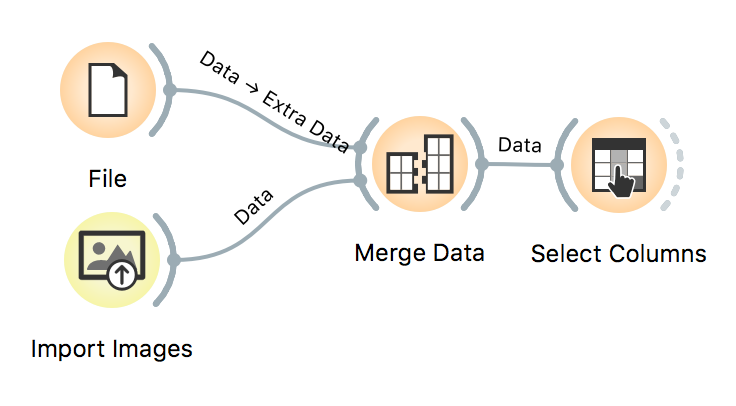
\includegraphics[scale=0.6]{intermediate-workflow.png}
\end{wrapfigure}

First, we load images with \widget{Import Images} from the Image Analytics add-on. Our images are organized, each type of amphora being in it own folder. Folders will be treated as categories upon loading. This means each image will get a special label with the name of the folder - the target variable.

Second, we have metadata belonging to each subtype of amphora (Dressel 6b, Gauloise 13, etc.). Load this with \widget{File} and join the two tables with \widget{Merge Data}. The widget should automatically recognize the attribute to merge by, but it case it doesn't, set both to \textit{image name}. Finally, we will use \widget{Select Columns} to put all the metadata to metas. Remember, our aim is to classify amphorae based on their image, not their description.

\begin{figure*}[h]
    \centering
    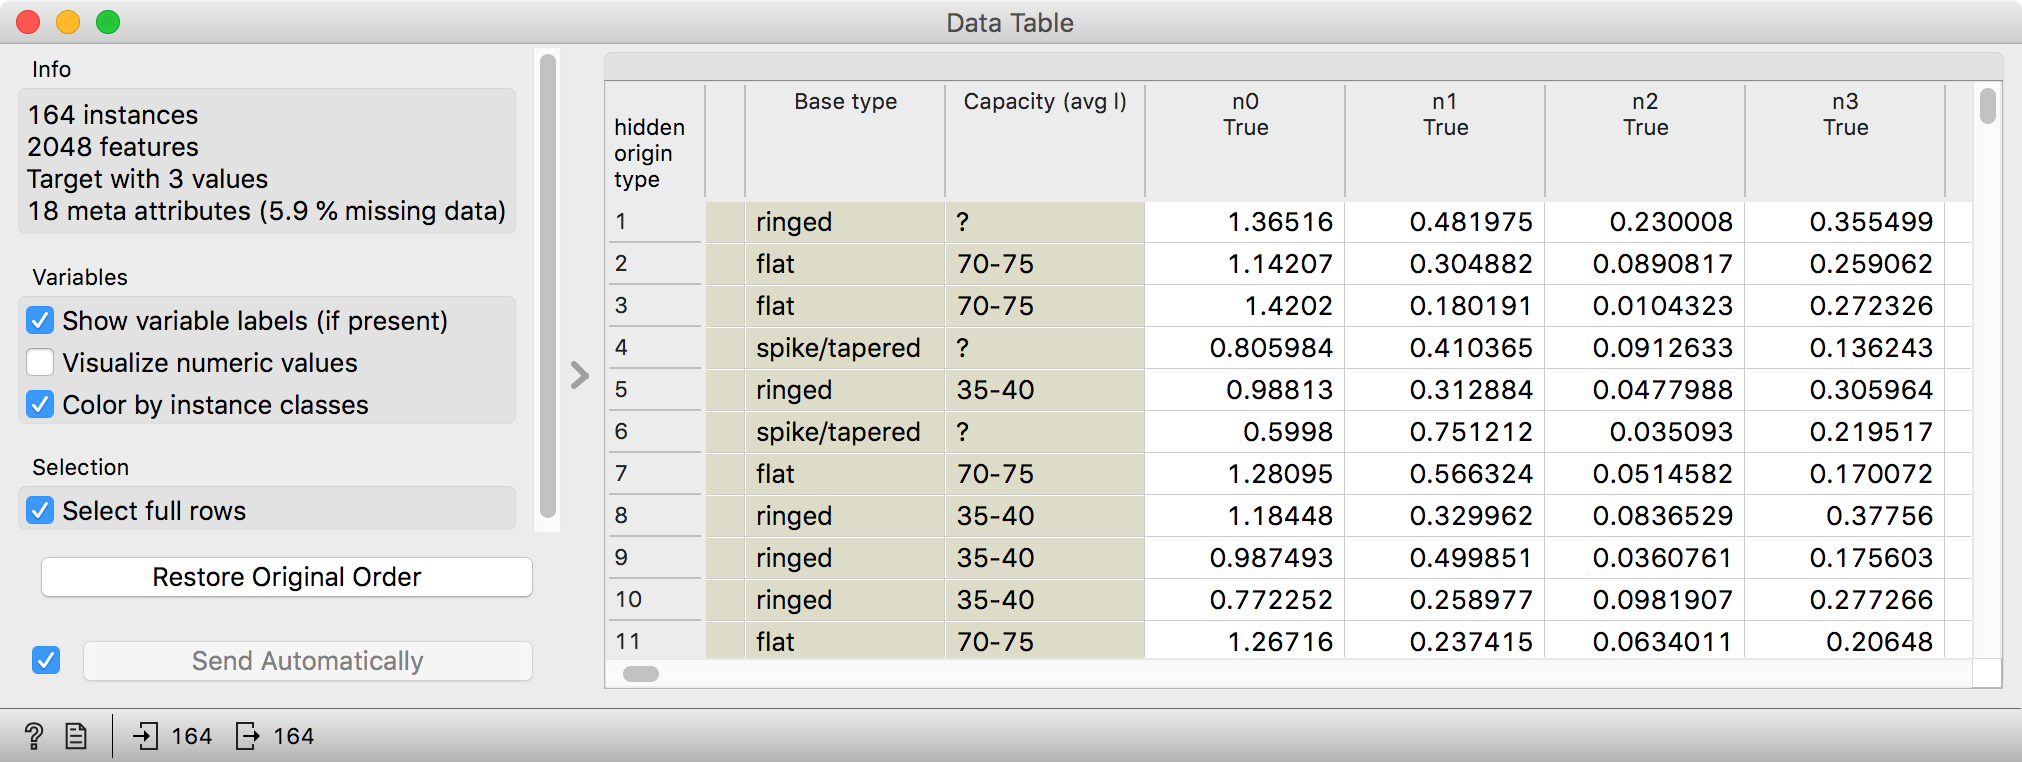
\includegraphics[width=\textwidth]{embeddings.png}
    \caption{$\;$} % empty caption for proper page setting
\end{figure*}

But machine learning works with numbers and images are not numbers, but complex objects. We need a way to transform images to a numeric description. We will use \widget{Image Embedding}, a widget that uses pre-trained deep models to infer image profiles. A common embedder is Google's Inception v3, which we will use for this exercise. Finally, we have our numbers! Specifically, a 2048-dimensional vector for each image.

Now, we can train a few classifiers. Common models for image classification are \widget{kNN}, \widget{Logistic Regression}, and \widget{SVM}, so let's use these. It looks like SVM has the highest AUC score, but Logistic Regression performs the best in other metrics.

\begin{figure}[h]
    \centering
    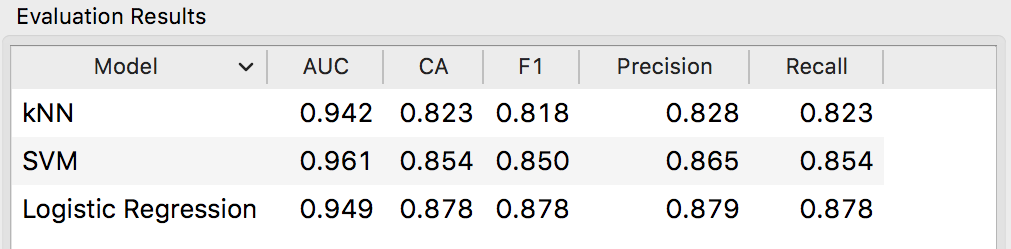
\includegraphics[scale=0.5]{test-and-score.png}
    \caption{$\;$} % empty caption for proper page setting
\end{figure}

\subsection{Assignment}

\begin{itemize}
    \item Observe \widget{Confusion Matrix} and determine which model is better to use in practice and why.
    \item Which type of amphorae is the most difficult to predict? How could we improve the performance? Select different misclassifications in Confusion Matrix and explore them in Image Viewer.
    \item There are three new images to predict. Use amphorae-predict and load it with Import Images. Pass it to Image Embedding, then use Predictions and the chosen model to predict image type. How accurate is the model? Would you use it in practice? Why (not)?
\end{itemize}

\begin{figure*}[h]
    \centering
    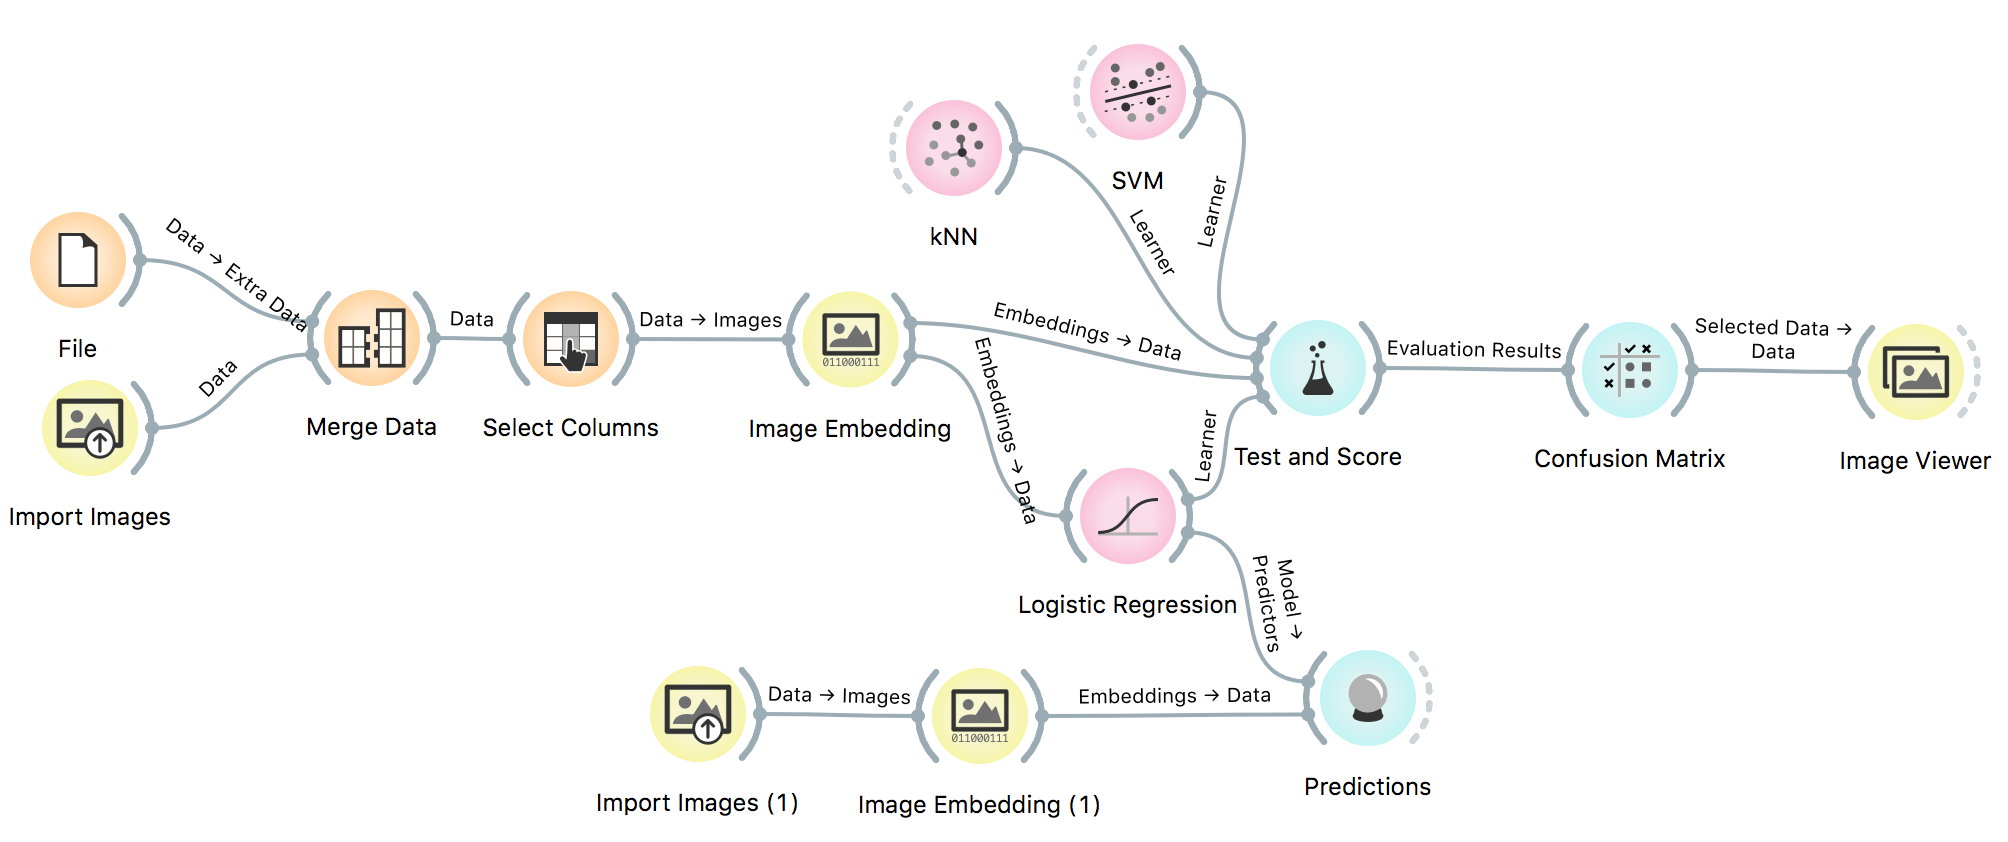
\includegraphics[width=\textwidth]{final-workflow.png}
    \caption{$\;$} % empty caption for proper page setting
\end{figure*}
